\documentclass[task=1]{exercise}
\usepackage{enumitem}
\usepackage{schule}
\usepackage{harpoon}

\newcommand\SJ{Schuljahr 22/23}

\newcommand\makeGlobalHeader[4]{
  \setgroup{#1\\#2}
  \settitle[#4]{#3}
  \addstudent{Datum:}
  \addstudent{~}
}

\newcommand\stufe{Kursstufe}
\newcommand\topic{Elektrostatik}

\newcommand\makeHeader[2]{
  \makeGlobalHeader{\topic}{\stufe}{#1}{#2}
}


\makeHeader{Widerstand}{Wiederholung}

\renewcommand{\vec}{\overrightharp}

\begin{document}
  \task[Definition Widerstand]
  \begin{enumerate}[label=\textnormal{\alph*)}]
    \item Gegeben sei die Spannung $U$ und der Strom $I$. Wie ist der Widerstand $R$ definiert?\\~\\
    \item Ergänze die Lücken:\\~\\
    Wenn der Strom $I$ gleich bleibt, dann gilt: Je größer die Spannung $U$, desto \luecke{3cm} der Widerstand $R$.\\~\\
    Wenn die Spannung $U$ gleich bleibt, dann gilt: Je größer der Strom $I$, desto \luecke{3cm} der Widerstand $R$.
    \item Was ist die Einheit der Spannung $U$, des Stromes $I$ und des Widerstandes $R$?\\~\\
  \end{enumerate}
  
  \task[Messreihen interpretieren]
  \begin{enumerate}[label=\textnormal{\alph*)}]
   \item Gegeben sei folgende Messreihe für Konstantandraht mit einer Dicke von $0{,}1$ mm und 50\,cm Länge. Vervollständige die letzte Zeile.\\~\\
   \begin{tabular}{|l|c|c|c|c|c|c|}\hline
    $U$ in V  ${\color{white} \displaystyle\frac{U}{I}}$& 0 & 1 & 2 & 3 & 4 & 5 \\\hline
    $I$ in A  ${\color{white} \displaystyle\frac{U}{I}}$& 0 & 0,03 & 0,06 & 0,10 & 0,13 & 0,15 \\\hline
    $R = \displaystyle\frac{\color{white} U}{\color{white} I}$ in $\displaystyle\frac{\color{white} U}{\color{white} I}$ & n.d. & ~~~~~~~~~ & ~~~~~~~~~ & ~~~~~~~~~ & ~~~~~~~~~ & ~~~~~~~~~ \\\hline
   \end{tabular}~\\~\\
   \item Gegeben sei folgende Messreihe für Konstantandraht mit einer Dicke von $0{,}2$ mm und 50\,cm Länge. Vervollständige die letzte Zeile.\\~\\
   \begin{tabular}{|l|c|c|c|c|c|c|}\hline
    $U$ in V  ${\color{white} \displaystyle\frac{U}{I}}$& 0 & 1 & 2 & 3 & 4 & 5 \\\hline
    $I$ in A  ${\color{white} \displaystyle\frac{U}{I}}$& 0 & 0,12 & 0,24 & 0,36 & 0,49 & 0,64 \\\hline
    $R = \displaystyle\frac{\color{white} U}{\color{white} I}$ in $\displaystyle\frac{\color{white} U}{\color{white} I}$ & n.d. & ~~~~~~~~~ & ~~~~~~~~~ & ~~~~~~~~~ & ~~~~~~~~~ & ~~~~~~~~~ \\\hline
   \end{tabular}~\\~\\
   \item Ergänze die Lücken:\\~\\
   Je dicker der Draht, desto \luecke{3cm} der Widerstand und desto \luecke{3cm} die Stromstärke.\\~\\
   Je dünner der Draht, desto \luecke{3cm} der Widerstand und desto \luecke{3cm} die Stromstärke.
   \newpage
   \item Zeichne die Messwerte aus a) und b) in das Diagramm ein, sowie eine Ausgleichsgerade für a) in blau und für b) in rot.\\~\\~\\~\\
   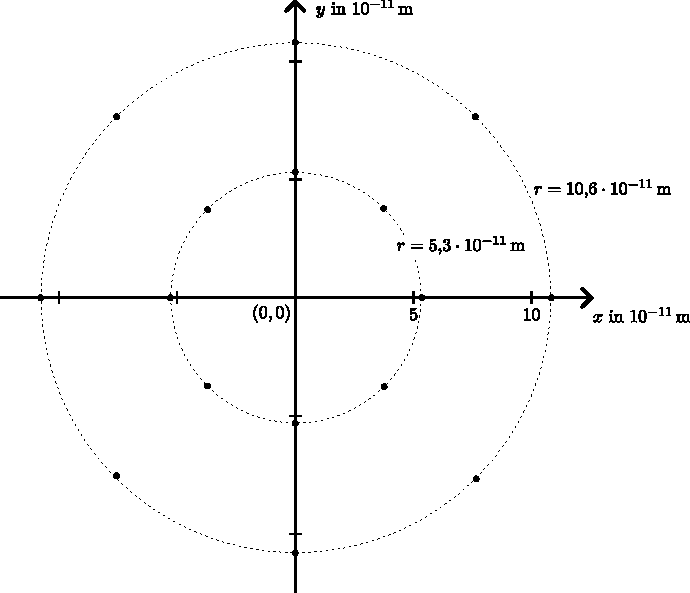
\includegraphics{images/diagram.pdf}
  \end{enumerate}

  \end{document}
